\subsection{CommonSenseQA}
{{\footnotesize
\noindent CommonsenseQA is a challenging multiple-choice QA dataset built from ConceptNet,
requiring models to apply commonsense knowledge to select the correct answer 
among five choices.


\begin{description}[labelwidth=4cm, labelsep=1em, leftmargin=4cm, itemsep=0.1em, parsep=0em]
  \item[date:] 2019-11-20
  \item[version:] 1
  \item[last\_updated:] 2019-11-20
  \item[expired:] false
  \item[valid:] yes
  \item[valid\_date:] 2019-11-20
  \item[url:] \href{https://paperswithcode.com/paper/commonsenseqa-a-question-answering-challenge}{https://paperswithcode.com/paper/commonsenseqa-a-question-answering-challenge}
  \item[doi:] 10.48550/arXiv.1811.00937
  \item[domain:] NLP; Commonsense
  \item[focus:] Commonsense question answering
  \item[keywords:]
    - ConceptNet
    - multiple-choice
    - adversarial
  \item[licensing:] MIT
  \item[task\_types:]
    - Multiple choice
  \item[ai\_capability\_measured:]
    - Commonsense reasoning and knowledge integration
  \item[metrics:]
    - Accuracy
  \item[models:]
    - BERT-large
    - RoBERTa
    - GPT-3
  \item[ml\_motif:]
    - Commonsense question answering
  \item[type:] Benchmark
  \item[ml\_task:]
    - Supervised Learning
  \item[solutions:] 2
  \item[notes:] Baseline 56\%, human 89\%
  \item[contact.name:] Alon Talmor, Jonathan Herzig, Nicholas Lourie, Jonathan Berant
  \item[contact.email:] Unknown
  \item[datasets.links.name:] CommonsenseQA Dataset (Hugging Face)
  \item[datasets.links.url:] \href{https://huggingface.co/datasets/commonsense\_qa}{https://huggingface.co/datasets/commonsense\_qa}
  \item[results.links.name:] Papers With Code Leaderboard for CommonsenseQA
  \item[results.links.url:] \href{https://paperswithcode.com/dataset/commonsenseqa}{https://paperswithcode.com/dataset/commonsenseqa}
  \item[fair.reproducible:] True
  \item[fair.benchmark\_ready:] True
  \item[id:] commonsenseqa
  \item[Citations:] \cite{talmor2019commonsenseqaquestionansweringchallenge}
\end{description}

{\bf Ratings:} ~ \\

\begin{tabular}{p{0.15\textwidth} p{0.07\textwidth} p{0.7\textwidth}}
\hline
Rating & Value & Reason \\
\hline
dataset & 5 & Public, versioned, and FAIR-compliant; includes metadata, splits, and licensing; well-integrated with HuggingFace and other ML libraries.
 \\
documentation & 5 & Given in paper.
 \\
metrics & 5 & Accuracy is a simple, reproducible metric aligned with task goals; no ambiguity in evaluation.
 \\
reference\_solution & 4 & Several baseline models (e.g., BERT, RoBERTa) are reported with scores; implementations exist in public repos, but not run with hardware constraints
 \\
software & 5 & All code given on Github site
 \\
specification & 4 & Task and format (multiple-choice QA with 5 options) are clearly defined; grounded in ConceptNet with consistent structure, though no hardware/system constraints are specified.
 \\
\hline
\end{tabular}

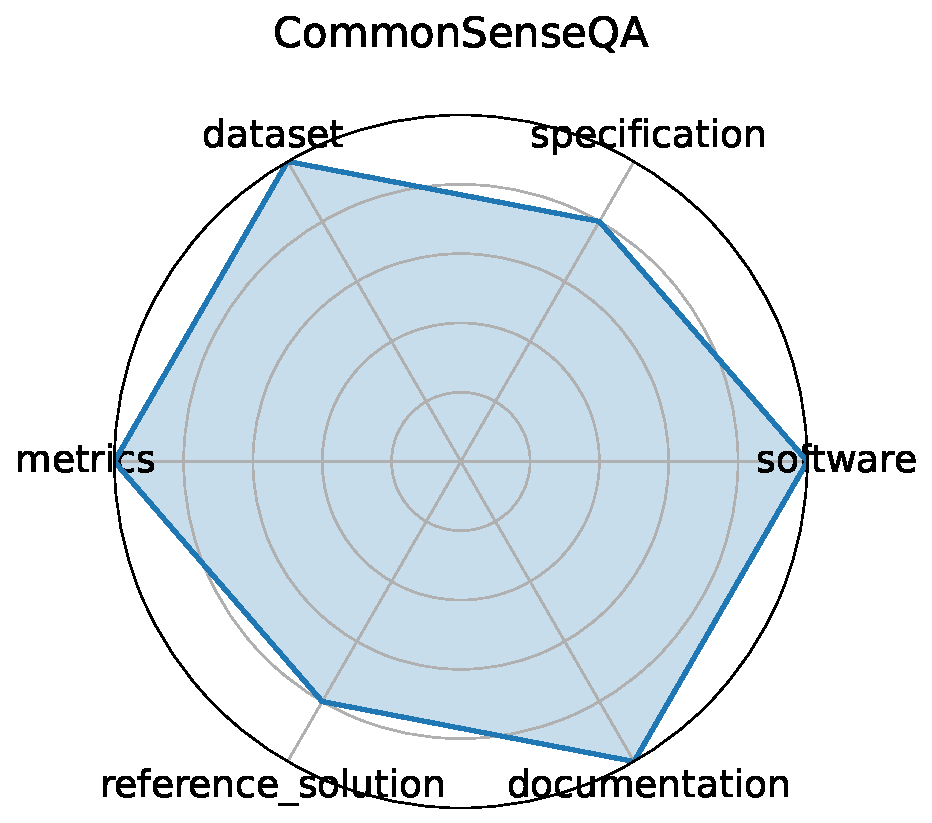
\includegraphics[width=0.2\textwidth]{commonsenseqa_radar.pdf}
}}
\clearpage